\documentclass[
  a4paper,
  12pt,
  spanish,
]{scrartcl}

% Párrafos
\setlength{\parindent}{18pt}

%-------------------------------------------------------------------------------
%	PAQUETES
%-------------------------------------------------------------------------------

% Idioma

\usepackage[es-noindentfirst]{babel}

% Matemáticas

\usepackage{amsmath, amsthm, amssymb}
\usepackage{mathtools}
\usepackage{commath}

% Fuentes personalizadas para utilizar con XeLaTeX o LuaLaTeX

\usepackage[no-math]{fontspec}
\setmainfont{Libertinus Serif}
\setsansfont{Libertinus Sans}
\setmonofont[Scale=.9]{Libertinus Mono}

\usepackage[math-style=TeX]{unicode-math}
\setmathfont{Libertinus Math}

% Configuración de microtype

\defaultfontfeatures{Ligatures=TeX,Numbers=Lining}
\usepackage[activate={true,nocompatibility},final,tracking=true,factor=1100,stretch=10,shrink=10]{microtype}
\SetTracking{encoding={*}, shape=sc}{0}

% Enlaces y colores

\usepackage{hyperref}
\usepackage[dvipsnames]{xcolor}
\definecolor{webgreen}{rgb}{0,0.5,0}
\hypersetup{
  colorlinks=true,
  citecolor=webgreen,
  urlcolor=Maroon,
  linkcolor=RoyalBlue
}

% Otros elementos de página

\usepackage{enumitem}
\setlist[enumerate]{leftmargin=*, itemsep=0pt}
\setlist[itemize]{leftmargin=*, itemsep=0pt}

\usepackage[labelfont=sc]{caption}

% Tikz

\usepackage{tikz}
\usetikzlibrary{babel}
\usepackage{float}

% Código

\usepackage{listings}
\lstset{
	basicstyle=\footnotesize\ttfamily,%
	breaklines=true,%
	captionpos=b,                    % sets the caption-position to bottom
  tabsize=2,	                   % sets default tabsize to 2 spaces
  frame=lines,
  numbers=left,
  stepnumber=1,
  aboveskip=12pt,
  showstringspaces=false,
}
\renewcommand{\lstlistingname}{Listado}

\usepackage{fancyvrb}

% Bibliografía

\usepackage[sorting=none, style=apa, isbn=true]{biblatex}
\DefineBibliographyStrings{spanish}{
  urlseen = {Consultado},
  retrieved = {Consultado},
}
\addbibresource{bibliografia.bib}

% Lorem ipsum

\usepackage{blindtext}

% Márgenes
\usepackage[bottom=3.125cm, top=2.5cm, left=4.5cm, right=4.5cm, marginparwidth=70pt]{geometry}

% Fuentes

\usepackage{textcase}

\newfontfamily{\sacshape}{Libertinus Serif}[
  WordSpace={1.8},
  LetterSpace={18.0}
]

\newfontfamily{\slscshape}{Libertinus Serif}[
  WordSpace={1.8},
  LetterSpace={6.0}
]

\DeclareRobustCommand{\spacedallcaps}[1]{{\linespread{1.3}\sacshape\MakeTextUppercase{#1}}}% WordSpace=1.8
\DeclareRobustCommand{\spacedlowsmallcaps}[1]{{\slscshape\MakeTextLowercase{#1}}}% WordSpace=1.8

% Cabeceras de sección

\RedeclareSectionCommands[beforeskip=-3ex,
afterskip=2ex]{section,subsection,subsubsection}
%\addtokomafont{section}{\normalfont\large\spacedallcaps}
%\setkomafont{section}{\normalfont\large\scshape}
\RedeclareSectionCommand[beforeskip=-9ex, font=\normalfont\large\scshape, tocentryformat=\normalfont\scshape]{section}
\addtokomafont{subsection}{\normalfont\normalsize\itshape}
\RedeclareSectionCommand[beforeskip=-6ex,tocentryformat=\normalfont\itshape]{subsection}
\addtokomafont{subsubsection}{\normalfont}
\RedeclareSectionCommand[beforeskip=-4ex]{subsubsection}
\addtokomafont{paragraph}{\normalfont\itshape}
%-------------------------------------------------------------------------------
%	TÍTULO
%-------------------------------------------------------------------------------

\newcommand{\horrule}[1]{\rule{\linewidth}{#1}}

%-------------------------------------------------------------------------------
%	CONTENIDO
%-------------------------------------------------------------------------------

\begin{document}

\begin{titlepage}
  \vspace*{4cm}

  \begin{flushleft}
    \Huge
    \spacedallcaps{Red Tor}
    \horrule{2pt}
  \end{flushleft}

  \vspace{2em}

  \begin{flushright}
    \large
    José María Martín Luque\\
    Antonio Martín Ruiz\\
    Daniel Pozo Escalona\vspace{1em}

    \textit{Seguridad y Protección de Sistemas Informáticos}

    Grado en Ingeniería Informática

    \textsc{Universidad de Granada}\vspace{1em}

    \today\vspace{.5em}
  \end{flushright}
\end{titlepage}

\newpage

{\hypersetup{hidelinks}
\tableofcontents
}

\newpage

\section{Introducción: ¿qué es Tor?}
% Común

Tor es una red superpuesta\footnote{
  Una red superpuesta es una red virtual de nodos enlazados lógicamente que utiliza la infraestructura de otra red existente \parencite[154]{kurose_computer_2013}.
} distribuida diseñada para anonimizar aplicaciones de baja latencia basadas en el protocolo TCP, como pueden ser un navegador web, una aplicación que implemente el protocolo SSH o un servicio de mensajería instantánea.
Los clientes escogen un camino a través de la red y crean un <<circuito>> en el que cada nodo ---o <<\textit{router} cebolla>>--- en dicho camino conoce su predecesor y sucesor pero no el resto de nodos del circuito.

\section{Estructura de la red Tor}
La red Tor está formada por nodos que se comunican mediante TLS sobre TCP/IP para mantener íntegra y oculta la información entre comunicaciones. Los nodos reciben el tráfico y lo reenvían.

El tráfico pasa por, al menos, tres nodos antes de llegar a su destino. Según la función que cumplen los nodos dentro del circuito podemos diferenciar tres tipos:

\begin{itemize}
\item Nodos medios. Reciben el tráfico y lo pasan a otro nodo. La presencia de los nodos medios es pública para toda la red Tor y cualquier usuario puede conectarse a ellos.
\item Nodos salida. Nodo final por el cuál pasa el tráfico antes de alcanzar su destino. Son también de acceso público para toda la red tor. La IP de estos nodos es interpretada por el receptor de información como la fuente del tráfico.
\item Puentes (\textit{bridges}). Nodos que no son públicos en la red Tor. Utilizados para evitar medidas de censura en países en los que regularmente se bloquean las IP de todos los nodos listados públicamente. Realizan la misma función que los nodos medios.
\end {itemize}

Existe además un servicio de directorio que publica la lista de nodos disponibles e información sobre ellos. Esta información es accesible a todos los nodos medios y todos los usuarios finales la usan para poder conectarse a la red. Existen una serie de nodos principales llamados \textit{autoridades de directorio} ---nodos confiables--- y nodos secundarios que actúan como \textit{caché} y \textit{backup} de los principales. Para dar fiabilidad al servicio de directorio las entradas son protegidas mediante firmas y solo la información proveniente de autoridades de directorio aprobadas son publicadas en la base de datos. Todo nodo nuevo de la red debe ser previamente aprobado, no existiendo un procedimiento automático para ello. Los administradores del servicio de directorio deben hacerlo manualmente.

\section{Enrutamiento cebolla}
% Antonio

Para el envío de tráfico a través de la red se utiliza un procedimiento llamado \textit{enrutamiento cebolla}. Esto es debido a cómo se acumulan capas de cifrado sobre el mensaje original. Veamos el procedimiento general y en apartados posteriores desarrollaremos más ampliamente los procedimientos criptográficos utilizados.

El emisor consulta su propia configuración y el directorio para obtener la información sobre como formar el circuito. Se seleccionan los nodos que serán utilizados. Por defecto cada circuito tiene tres nodos medios.

Se negocian las claves de cifrado con cada nodo. Se establecen claves simétricas mediante \textit{Diffie-Hellman}. El circuito se construye desde el punto de entrada. Los mensajes para negociar las claves entre el nodo \(n\) y el \(n+1\) se realiza retransmitiendo paquetes entre el emisor y retransmitiendo paquetes desde el nodo \(1\) hasta el \(n\), y de ahí al nodo \(n+1\). En cada paso los mensajes son cifrados con las claves previamente negociadas. Una vez establecidas las claves se puede enviar tráfico.

\begin{figure}[h]
  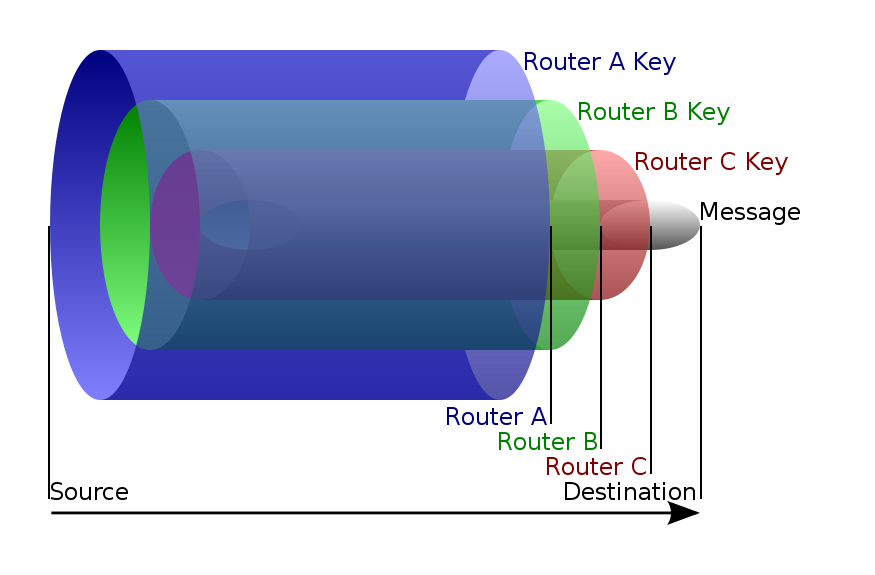
\includegraphics[width=\textwidth]{OR4.png}
  \caption{Representación visual del enrutamiento cebolla \parencite{wikipedia:hantwister_svg_2008}.}
  \label{fig:or4}
\end{figure}

Los paquetes se cifran con las claves recibidas en orden inverso: primero se cifra con la clave del último nodo, luego con la del penúltimo, y así hasta llegar al primero. Se envía el paquete resultante a través del circuito y a su paso por cada nodo se elimina la capa de cifrado correspondiente a dicho nodo. En la figura \ref{fig:or5} puede verse un esquema de un ejemplo de comunicación.

\begin{figure}[h]
  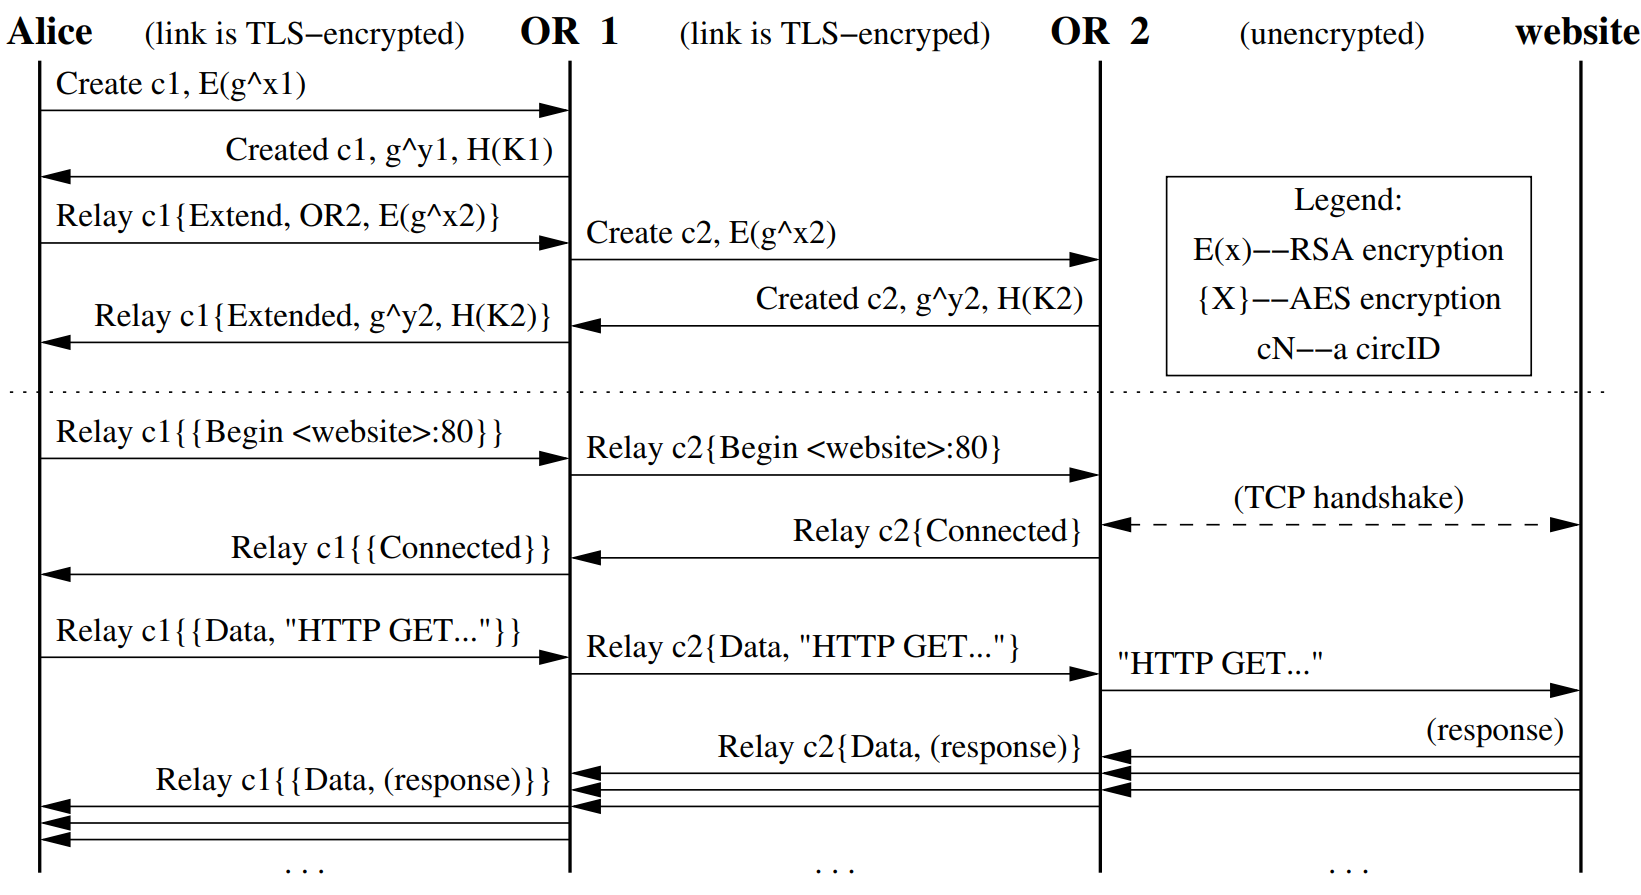
\includegraphics[width=\textwidth]{OR5.png}
  \caption{Diagrama representando un ejemplo de comunicación entre una usuaria, Alice, y una página web, pasando por dos nodos \parencite{dingledine_tor:_2004}.}
  \label{fig:or5}
\end{figure}

Puesto que solo el primer nodo conoce desde dónde proviene la información y sólo el nodo final conoce cuál es la información, no es posible saber quién la envía y qué se envía.

\section{Algoritmos de cifrado}
% Jose

Las conexiones entre dos repetidores en un circuito Tor, o entre el cliente y un repetidor utilizan el protocolo TLS/SSLv3 para la autentificación y el cifrado de los enlaces.
Se conoce como \textit{suite de cifrado} al conjunto de algoritmos utilizados al establecer una comunicación mediante TLS.
Dicha \textit{suite} suele incluir un algoritmo de intercambio de intercambio de claves, un algoritmo de cifrado en bloque y un algoritmo de código de autentificación de mensaje.
La especificación de Tor \parencite{dingledine_tor_2019} permite que el usuario elija una \textit{suite} de cifrado de entre una lista predefinida, aunque todas las implementaciones deben soportar como mínimo \texttt{TLS\_DHE\_RSA\_WITH\_AES\_128\_CBC\_SHA}.

Sin entrar en demasiados detalles, el protocolo TLS tiene dos fases: una primera en la que ambas partes establecen la conexión y se ponen de acuerdo en una clave compartida con la que cifrar la información (mediante el uso del algoritmo de intercambio de claves), y una segunda en la que proceden al intercambio de información en sí, utilizando para ello el algoritmo de cifrado en bloque \parencite{ibm_overview_2019}.

Para establecer la conexión TLS entre los nodos del circuito creado por el usuario se utiliza una implementación del protocolo de Diffie-Hellman.
Originalmente Tor utilizaba un protocolo de autentificación ---denominado posteriormente como TAP, \textit{Tor Authentication Protocol}--- que implementaba Diffie-Hellman sobre el grupo finito \(Z_p\), junto a RSA para calcular un conjunto de claves que ambos nodos comparten \parencite{dingledine_tor:_2004}.

Análisis posteriores \parencite{hutchison_security_2006} llegaron a la conclusión de que TAP tenía deficiencias, lo que condujo a la creación de un nuevo protocolo denominado \textit{ntor} y que se introdujo en la versión \texttt{0.2.4.8-alpha} de Tor.
Este nuevo protocolo utiliza ECDH (\textit{Elliptic Curve Diffie-Hellman}), que implementa el protocolo de Diffie-Hellman para un grupo curvas elípticas, en lugar de un grupo \(Z_p\). Tor en concreto utiliza el grupo Curve25519 \parencite{yung_curve25519:_2006}, que ofrece tamaños de clave de 128 bits.

Finalmente, una vez establecida la conexión TLS, se utiliza AES con claves de 128 bits para el cifrado de la información intercambiada entre dos nodos.

Como función \textit{hash}, se utiliza SHA-1 por defecto, aunque también se utilizan SHA256 y SHA3-256 en algunos puntos.

\subsection{Parámetros de los algoritmos}

La especificación de Tor describe los parámetros que se utilizan por defecto cuando se usa alguno de los algoritmos de cifrado descritos anteriormente, a saber: \begin{itemize}
  \item Para Diffie-Hellman sobre \(Z_p\) se utiliza como generador \(g=2\) y \(p\) es el primo seguro de 1024 bits descrito en \parencite{carrel_internet_1998}, cuyo valor es \[
    2^{1024} - 2^{960} - 1 + 2^{64} \cdot \left\lfloor (2^{894} \pi) + 129093 \right\rfloor.
  \]
  %y cuya representación hexadecimal se describe en la figura \ref{verb:primo-seguro}.
  % \begin{figure}[h]
  %   \centering
  %   \begin{BVerbatim}
  % FFFFFFFF FFFFFFFF C90FDAA2 2168C234 C4C6628B
  % 80DC1CD1 29024E08 8A67CC74 020BBEA6 3B139B22
  % 514A0879 8E3404DD EF9519B3 CD3A431B 302B0A6D
  % F25F1437 4FE1356D 6D51C245 E485B576 625E7EC6
  % F44C42E9 A637ED6B 0BFF5CB6 F406B7ED EE386BFB
  % 5A899FA5 AE9F2411 7C4B1FE6 49286651 ECE65381
  % FFFFFFFF FFFFFFFF
  %   \end{BVerbatim}
  %   \caption{Representación hexadecimal del primo}
  %   \label{verb:primo-seguro}
  % \end{figure}
  \item Para Diffie-Hellman con curvas elípticas se utiliza el grupo Curve25519, como ya se ha mencionado antes.
  \item Para RSA se utilizan claves de tamaño \(1024\) y un exponente fijo, \(65537\).
\end{itemize}

\section{Posibles ataques}
% Dani


%-------------------------------------------------------------------------------
%	BIBLIOGRAFÍA
%-------------------------------------------------------------------------------

\newpage
\printbibliography

\end{document}
